% \subsection{ỨNG DỤNG NGUYÊN HÀM TRONG THỰC TIỄN}
\begin{dang}{Ứng dụng trong bài toán thực tiễn}
	Giả sử $v(t)$ là vận tốc của vật $ {M}$ tại thời điểm $t$ và $s(t)$ là quãng đường vật đi được sau khoảng thời gian $t$ tính từ lúc bắt đầu chuyển động. Ta có mối liên hệ giữa $s(t)$ và $v(t)$ như sau.
	\begin{itemize}
		\item  Đạo hàm của quãng đường là vận tốc $s'(t)=v(t)$.
		\item  Nguyên hàm của vận tốc là quãng đường $s(t)=\displaystyle\int v(t)  \mathrm{\,d} t$.
	\end{itemize}
	Nếu gọi $a(t)$ là gia tốc của vật M thì ta có mối liên hệ giữa $v(t)$ và $a(t)$ như sau.
	\begin{itemize}
		\item Đạo hàm của vận tốc là gia tốc $v'(t)=a(t)$.
		\item Nguyên hàm của gia tốc là vận tốc $v(t)=\displaystyle\int\limits a(t)  \mathrm{\,d} t$.
	\end{itemize}
\end{dang}
% \TN
\Opensolutionfile{ans}[ans/ans2-C4B1CD4-D1]
\begin{ex}%[2D4V1-6]
	Một ô tô đang chạy với vận tốc $20$ m/s thì người lái đạp phanh. Sau khi đạp phanh, ô tô chuyển động chậm dần đều với vận tốc $v(t)=-40t+20$ m/s, trong đó $t$ là khoảng thời gian tính bằng giây kể từ lúc bắt đầu đạp phanh. Gọi  $s(t)$ là quãng đường xe ô tô đi được trong thời gian $t$  (giây) kể từ lúc đạp phanh. Hỏi từ lúc đạp phanh đến khi dừng hẳn, ô tô còn di chuyển bao nhiêu mét?
	\choice{$5$ cm}{$7{,}5$ m}{$\dfrac{5}{2}$ m}{\True $5$ m}
	\loigiai{
		Ta có $v(t)=-40t+20$.\\
		Suy ra $s(t)=\displaystyle\int v(t)\mathrm{\,d}t=\displaystyle\int (-40t+20)\mathrm{\,d}t=-20t^2+20t+C$.\\
		Chọn $t=0$ suy ra $s(0)=0\Rightarrow C=0$.\\
		Khi đó $s(t)=-20t^2+20t$.\\
		Khi xe dừng hẳn $v(t)=0\Leftrightarrow -40t+20=0\Leftrightarrow t=0{,}5$.\\
		Từ lúc đạp phanh đến khi dừng hẳn, ô tô còn di chuyển được\\ $s(0{,}5)=-20\cdot (0{,}5)^2+20\cdot 0{,}5=5$ m.
	}
\end{ex}
\Opensolutionfile{ans}[ans/ansMyLT]
%\begin{ex}%[2D4H1-6]
%Một ô tô đang chạy với vận tốc $20$ m/s thì người người đạp phanh. Sau khi đạp phanh, ô tô chuyển động chậm dần đều với vận tốc $v(t)=-40t+20$ m/s, trong đó $t$ là khoảng thời gian tính bằng giây kể từ lúc bắt đầu đạp phanh. Gọi $s(t)$ là quãng đường xe ô tô đi được trong thời gian $t$ (giây) kể từ lúc đạp phanh. Hỏi từ lúc đạp phanh đến khi dừng hẳn, ô tô còn di chuyển bao nhiêu mét?
%\choice
%{$5$ cm}
%{$7,5$ m}
%{$\dfrac{5}{2}$ m}
%{\True $5$ m}
%\begin{center}
%	\color{red}HÌNH Ở ĐÂY
%\end{center}
%\loigiai{
	%Ta có $v(t)=-40t+20$\\
	%$\Rightarrow s(t)=\displaystyle\int{v(t)}dt=\displaystyle\int{\left(-40t+20\right)}dt=-20t^2+20t+C$\\
	%$\Rightarrow s(t)=-20t^2+20t+C$\\
	%Chọn $t=0\Rightarrow s(0)=0$ $\Rightarrow C=0$\\
	%$\Rightarrow s(t)=-20t^2+20t$\\
	%Khi xe dừng hẳn thì $v(t)=0\Leftrightarrow-40t+20=0\Rightarrow t=0{,}5$.\\
	%từ lúc đạp phanh đến khi dừng hẳn, ô tô còn di chuyển được:\\ $s\left(0{,}5\right)=-20\left(0{,}5\right)^2+20\left(0{,}5\right)=5$ m.}
%\end{ex}

\begin{ex}%[2D4H1-6]
	Bạn Minh Hiền ngồi trên máy bay đi du lịch thế giới với vận tốc chuyển động của máy báy là $v(t)=3t^2+5$ (m/s). Quãng đường máy bay bay từ giây thứ $4$ đến giây thứ $10$ là
	\begin{center}
		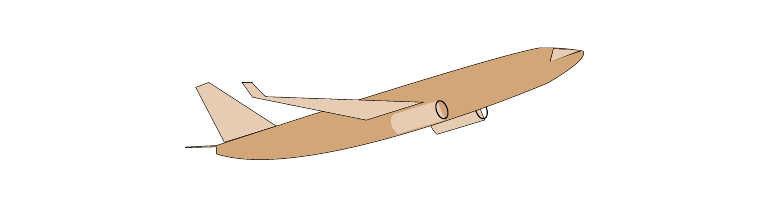
\begin{tikzpicture}
			\clip (-4.5,-1) rectangle (4.5,1);
			%\path (0,0) node[opacity=.5,scale=.3] {\includegraphics{6}};
			%\draw[gray!50] (-4,-2) grid (4,2);
			\begin{pgfinterruptboundingbox}
				%Đuôi máy bay
				\def\D{ (-2,-.45)--(-2.36,.24)--(-2.2,.3)--(-1.35,-.25)--cycle
					;}
				\draw \D;
				\fill[brown!40!] \D;
				%Quạt máy bay
				\def\Q{ (.15,-.1)
					..controls +(-140:0.1) and +(140:0.1) .. (.2,-.35)--(.8,-.17)--(.7,.07)--cycle;}
				\draw \Q;
				\draw[xshift=.5cm] \Q;
				\fill[brown!40!,xshift=.5cm] \Q;
				%---------elip2
				\draw[rotate=-70,xshift=-.23cm,yshift=1.27cm] (.7,-.1) ellipse (.12cm and .07cm);
				%Thân máy bay
				\def\T{ (-2.1,-.5)
					..controls +(40:0) and +(-170:0.7) .. (2,.74)
					..controls +(-40:0) and +(170:0.3) .. (2.55,.7)
					..controls +(-150:0) and +(30:.65) .. (2.1,.3)
					..controls +(-150:0) and +(-18:1.25) .. (-2.1,-.6)
					..controls +(90:0) and +(-90:0) .. (-2.1,-.51)
					-- (-2.5,-.52)--cycle;
				}
				\draw \T;
				\fill[brown!70!] \T;
				%Cánh máy bay
				\def\C{ (.5,.05)
					..controls +(170:0) and +(-10:0) .. (-1.48,.12)
					..controls +(-80:0) and +(170:0.02) .. (-1.65,.3)
					..controls +(180:0) and +(0:0) .. (-1.77,.3)
					..controls +(-80:0) and +(110:0) .. (-1.64,.12)
					..controls +(-35:0) and +(145:0) .. (-.2,-.17)
					--cycle;}
				\draw \C;
				\fill[brown!40!] \C;
				%Quạt sau
				\fill[brown!40!] \Q;
				
				%----elip 1
				\draw[rotate=-70,xshift=-.4cm,yshift=.8cm] (.7,-.1) ellipse (.12cm and .07cm);
				%Ô cửa
				\draw (2.18,0.73)--(2.5,0.7)--(2.14,0.58)--cycle;
				\fill[brown!40!](2.18,0.73)--(2.51,0.71)--(2.14,0.57)--cycle;
			\end{pgfinterruptboundingbox}
		\end{tikzpicture}
	\end{center}
	\choice
	{$36$ m}
	{$252$ m}
	{$1134$ m}
	{\True $966$ m}
	
	\loigiai{
		Ta có $v(t)=3t^2+5$.\\
		$\Rightarrow s(t)=\displaystyle\int{v(t)\mathrm{\,d}t}=\displaystyle\int{\left(3t^2+5\right)} \mathrm{\,d}t=t^3+5t+C$.\\
		$\Rightarrow s(t)=t^3+5t+C$.\\
		Chọn $t=0\Rightarrow s(0)=0 \Rightarrow C=0$.\\
		$\Rightarrow s(t)=t^3+5t$.\\
		Quãng đường máy bay bay từ giây thứ $4$ là $s(4)=4^3+5\cdot4=84$ (m).\\
		Quãng đường máy bay bay từ giây thứ $10$ là $s\left(10\right)=10^3+5\cdot 10=1050$ (m).\\
		Quãng đường máy bay bay từ giây thứ $4$ đến giây thứ $10$ là $s(10)-s(4)=966$ (m).}
\end{ex}

\begin{ex}%[2D4H1-6]
	Một ô tô đang chạy với vận tốc $12$ m/s thì người lái đạp phanh; từ thời điểm đó, ô tô chuyển động chậm dần đều với vận tốc $v(t)=-6t+12$ (m/s), trong đó $t$ là khoảng thời gian tính bằng giây kể từ lúc đạp phanh. Hỏi từ lúc đạp phanh đến khi ô tô dừng hẳn, ô tô còn di chuyển được bao nhiêu mét?
	\choice
	{$24$ m}
	{\True $12$ m}
	{$6$ m}
	{$0{,}4$ m}
	\loigiai{
		Ta có 
		\begin{eqnarray*}
			& & v(t)=-6t+12\\
			&\Rightarrow & s(t)=\displaystyle\int{v(t) \mathrm{\,d}t}\\
			&\Leftrightarrow &  s(t)=\displaystyle\int (-6t+12)\mathrm{\,d}t\\
			&\Leftrightarrow &  s(t)=-3t^2+12t+C.
		\end{eqnarray*}
		Chọn $t=0\Rightarrow s(0)=0 \Rightarrow C=0\Rightarrow s(t)=-3t^2+12t$.\\
		Khi xe dừng hẳn thì $v(t)=0\Leftrightarrow-6t+12=0\Rightarrow t=2$.\\
		Từ lúc đạp phanh đến khi ô tô dừng hẳn thì ô tô còn di chuyển được quãng đường là
		$$S=s(2)-s(0)=s(2)=-3\cdot 2^2 +12\cdot 2 =12\text{ (m).}$$
	}
\end{ex}

\begin{ex}%[2D4H1-6]
	Một ô tô đang chạy với vận tốc $36$ km/h thì tăng tốc chuyển động nhanh dần đều với gia tốc $a(t)=1+\dfrac{t}{3}$ (m/s$^2$) tính quãng đường ô tô đi được sau $6$ giây kể từ khi ô tô bắt đầu tăng tốc.
	\choice
	{\True $S=90$ m}
	{$S=246$ m}
	{$S=58$ m}
	{$S=100$ m}
	\loigiai{
		Đổi $36$ km/h $= 36\cdot \dfrac{1000}{3600}=10$ m/s.\\
		Ta có $a(t)=1+\dfrac{t}{3}$.\\
		$\Rightarrow v(t)=\displaystyle\int{a(t) \mathrm{\,d}t}=\displaystyle\int \left(1+\dfrac{t}{3}\right) \mathrm{\,d}t=t+\dfrac{1}{6}t^2+C$.\\
		Từ lúc bắt đầu tăng tốc thì vận tốc của xe là $10$ m/s nên ta có 
		\begin{eqnarray*}
			& & v(0)=10\\
			&\Rightarrow & C=10\\
			&\Rightarrow & v(t)=t+\dfrac{1}{6}t^2+10\\
			&\Rightarrow & s(t)=\displaystyle\int{v(t) \mathrm{\,d}t}\\
			&\Rightarrow & s(t)=\displaystyle\int (t+\dfrac{1}{6}t^2+10)\\
			&\Rightarrow & s(t)=\dfrac{t^2}{2}+\dfrac{t^3}{18}+10t + C_1.
		\end{eqnarray*}
		Quãng đường tính từ lúc xe bắt đầu tăng tốc nên $s(0)=0 \Rightarrow C_1=0$.\\
		Vậy $s(6)=\dfrac{6^2}{2}+\dfrac{6^3}{18}+10\cdot 6 =90$ (m).
	}
\end{ex}

\begin{ex}%[2D4H1-6]
	Một ca nô đang chạy trên hồ Tây với vận tốc $20$ m/s thì hết xăng; từ thời điểm đó, ca nô chuyển động chậm dần đều với vận tốc $v(t)=-5t+20$ (m/s), trong đó $t$ là khoảng thời gian tính bằng giây, kể từ lúc hết xăng. Hỏi từ lúc hết xăng đến lúc ca nô dừng hẳn thì ca nô đi được bao nhiêu mét?
	\choice
	{$10$ m}
	{$20$ m}
	{$30$ m}
	{\True $40$ m}
	\loigiai{
		Ta có $v(t)=-5t+20$.\\
		$\Rightarrow s(t)=\displaystyle\int{v(t)} \mathrm{\,d}t=\displaystyle\int{\left(-5t+20\right)} \mathrm{\,d}t=-\dfrac{5}{2}t^2+20t+C$.\\
		Chọn $t=0\Rightarrow s(0)=0 \Rightarrow C=0$. Suy ra $s(t)=-\dfrac{5}{2}t^2+20t$.\\
		Khi xe dừng hẳn thì $v(t)=0\Leftrightarrow-5t+20=0\Rightarrow t=4$ (s).\\
		Từ lúc đạp phanh đến khi dừng hẳn, ô tô còn di chuyển được $s = -\dfrac{5}{2}\cdot 4^2+20\cdot 4=40$ (m).
	}
\end{ex}

\begin{ex}%[2D4H1-6]
	Một vật chuyển động với vận tốc $10$ m/s thì tăng tốc với gia tốc được tính theo thời gian $t$ là $a(t)=3t+t^2$ (m$^2$/s). Tính quãng đường vật đi được trong $10$s kể từ khi bắt đầu tăng tốc.
	\choice
	{$\dfrac{130}{3}$ m}
	{$\dfrac{310}{3}$ m}
	{$\dfrac{3400}{3}$ m}
	{\True $\dfrac{4300}{3}$ m}
	\loigiai{
		Ta có $a(t)=3t+t^2$\\
		$\Rightarrow v(t)=\displaystyle\int{a(t) \mathrm{\,d}t}=\displaystyle\int (3t+t^2) \mathrm{\,d}t=\dfrac{3}{2}t^2+\dfrac{1}{3}t^3+C$.\\
		Từ lúc bắt đầu tăng tốc thì vận tốc của xe là $10$ m/s nên ta có \\ 
		$v(0)=10 \Rightarrow C=10$.\\
		$\Rightarrow v(t)=\dfrac{3}{2}t^2+\dfrac{1}{3}t^3+10$.\\
		$\Rightarrow s(t)=\displaystyle\int{v(t) \mathrm{\,d}t}=\displaystyle\int (\dfrac{3}{2}t^2+\dfrac{1}{3}t^3+10) \mathrm{\,d}t=\dfrac{1}{2}t^3+\dfrac{1}{12}t^4+10t+C_1$.\\
		Quãng đường tính từ lúc xe bắt đầu tăng tốc nên $s(0)=0 \Rightarrow C_1=0$.\\
		Vậy $s(10)=\dfrac{1}{2}\cdot 10^3+\dfrac{1}{12}\cdot 10^4+10\cdot 10=\dfrac{4300}{3}$ m.
	}
\end{ex}

\begin{ex}%[2D4H1-6]
	Tại một nơi không có gió, một chiếc khí cầu đang đứng yên ở độ cao $162$ m so với mặt đất đã được phi công cài đặt cho nó chế độ chuyển động đi xuống. Biết rằng, khí cầu đã chuyển động theo phương thẳng đứng với vận tốc tuân theo quy luật $v(t)=10t-t^2$, trong đó $t$ (phút) là thời gian tính từ lúc bắt đầu chuyển động, $v(t)$ được tính theo đơn vị mét/phút (m/p). Nếu như vậy thì khi bắt đầu tiếp đất vận tốc $v$ của khí cầu là
	\choice
	{$5$ m/p}
	{$7$ m/p}
	{\True $9$ m/p}
	{$3$ m/p}
	\loigiai{
		Ta có $v(t)=10t-t^2$.\\
		$\Rightarrow s(t)=\displaystyle\int{v(t) \mathrm{\,d}t}=\displaystyle\int (10t-t^2) \mathrm{\,d}t=5t^2-\dfrac{1}{3}t^3+C$.\\
		Từ lúc bắt đầu giảm độ cao thì khinh khí cầu ở độ cao $162$ m nên ta có \\ 
		$s(0)=0 \Rightarrow C=0\Rightarrow s(t)=5t^2-\dfrac{1}{3}t^3$.\\
		mà $s(t)= 162 \Rightarrow 5t^2-\dfrac{1}{3}t^3=162 \Leftrightarrow t=9$ (s).\\
		Suy ra vận tốc khi chạm đất của khinh khí cầu là
		$$v(9)= 10\cdot 9 -9^2=9 \text{ (m/p)}.$$
	}
\end{ex}

\begin{ex}%[2D4H1-6]
	Một viên đạn được bắn lên theo phương thẳng đứng với vận tốc ban đầu là $25$ m/s, gia tốc trọng trường là $9{,}8$ m/s$^2$. Quãng đường viên đạn đi được từ lúc bắn cho đến khi chạm đất gần bằng kết quả nào nhất trong các kết quả sau?
	\choice
	{$30{,}78$ m}
	{\True $31{,}89$ m}
	{$32{,}43$ m}
	{$33{,}88$ m}
	\loigiai{
		Ta có $a(t)=-9{,}8$ (m/s$^2$).\\
		$\Rightarrow v(t)=\displaystyle\int{a(t) \mathrm{\,d}t}=\displaystyle\int (-9{,}8) \mathrm{\,d}t=-9{,}8t+C$.\\
		Từ lúc bắt đầu bắn viên đạn thì viên đạn có vận tốc $25$ m/s nên ta có\\
		$v(0)=25 \Rightarrow C=25 \Rightarrow v(t)=-9{,}8t+25$.\\ 
		$\Rightarrow s(t)=\displaystyle\int{v(t) \mathrm{\,d}t}=\displaystyle\int (-9{,}8t+25) \mathrm{\,d}t=-4{,}9t^2+25t+C_1$.\\
		Ta có $s(0)=0 \Rightarrow C_1=0$.\\
		$s(t)=-4{,}9t^2+25t$.\\
		Tới khi vận tốc viên đạn bằng không thì ta có $v(t)=0 \Rightarrow -9{,}8t+25=0 \Leftrightarrow t \approx 2{,}55$ s.
		Suy ra quãng đường viên đạn đi được từ lúc bắn cho đến khi chạm đất là\\
		$S= 2\cdot (-4{,}9\cdot (2{,}55)^2+25\cdot 2{,}55) \approx 31{,}89$ m.
	}
\end{ex}

\begin{ex}%[2D4H1-6]
	Trong một đợt xả lũ, nhà máy thủy điện đã xả lũ trong $40$ phút với tốc độ lưu lượng nước tại thời điểm $t$ giây là $h'(t)=10t+500$ (m$^3$/s). Hỏi sau thời gian xả lũ trên thì hồ thoát nước của nhà máy đã thoát đi một lượng nước là bao nhiêu?
	\choice
	{$5\cdot 10^4$ m$^3$}
	{$4\cdot 10^6$ m$^3$}
	{\True $3\cdot 10^7$ m$^3$}
	{$6\cdot 10^6$ m$^3$}
	\loigiai{
		Ta có $h'(t)=10t+500$.\\
		$\Rightarrow h(t)=\displaystyle\int{\left(10t+500\right)}\mathrm{\,dx}=5t^2+500t+C$.\\
		$\Rightarrow h(t)=5t^2+500t+C$.\\
		Chọn $t=0\Rightarrow h(0)=0\Rightarrow C=0$.\\
		$\Rightarrow h(t)=5t^2+500t$.\\
		Thủy điện đã xả lũ trong $40$ phút=$2400$ giây thì thoát đi một lượng nước là
		$$h\left(2400\right)=5\cdot 2400^2+500\cdot 2400=3\cdot 10^7\text{ (m$^3$)}.$$
	}
\end{ex}

\begin{ex}%[2D4H1-6]
	Một bác thợ xây bơm nước vào bể chứa nước. Gọi $h(t)$ là thể tích nước bơm được sau $t$ giây. Cho $h'(t)=3a{t^2}+bt$ (m$^3$/s) và ban đầu bể không có nước. Sau $5$ giây thì thể tích nước trong bể là $150$ m$^3$. Sau $10$ giây thì thể tích nước trong bể là $1100$ m$^3$. Hỏi thể tích nước trong bể sau khi bơm được $20$ giây là bao nhiêu.
	\choice
	{\True $8400$ m$^3$}
	{$7400$ m$^3$}
	{$6000$ m$^3$}
	{$4200$ m$^3$}
	\loigiai{
		Ta có $h'(t)=3a{t^2}+bt$.\\
		$\Rightarrow h(t)=\displaystyle\int{\left(3a{t^2}+bt\right)} \mathrm{\,d}t=a{t^3}+\dfrac{1}{2}b{t^2}+C$.\\
		$\Rightarrow h(t)=a{t^3}+\dfrac{1}{2}b{t^2}+C$.\\
		Chọn $t=0\Rightarrow h(0)=0\Rightarrow C=0$.\\
		$\Rightarrow h(t)=a{t^3}+\dfrac{1}{2}b{t^2}$.\\
		Sau $5$ giây thì thể tích nước trong bể là $150$ m$^3$ là  $h(5)=150\Leftrightarrow 125a+\dfrac{25}{2}b=150$.\hfill(1)\\
		Sau $10$ giây thì thể tích nước trong bể là $1100$ m$^3$ là  $h(10)=1100\Leftrightarrow 1000a+50b=1100$.\hfill(2)\\
		Từ (1) và (2) ta có hệ  $\heva{
			&125a+\dfrac{25}{2}b=150\\
			&1000a+50b=1100
		}\Leftrightarrow \heva{&a=1\\&b=2.}$\\
		$\Rightarrow h(t)=t^3+t^2$.\\
		Thể tích nước trong bể sau khi bơm được $20$ giây là $h\left(20\right)=20^3+20^2=8400$ (m$^3$).}
\end{ex}

\begin{ex}%[2D4H1-6]
	Gọi $h(t)$ (m) là mực nước ở bồn chứa sau khi bơm nước được $t$ giây. Biết rằng $h'(t)=\dfrac{1}{5}\sqrt[3]{t}$ (m/s) và lúc đầu bồn không có nước. Tìm mức nước ở bồn sau khi bơm nước được $6$ giây (\textit{làm tròn kết quả đến hàng phần trăm}).
	\choice
	{$2{,}64$ m}
	{$1{,}22$ m}
	{$2{,}22$ m}
	{\True $1{,}64$ m}
	\loigiai{
		Ta có $h'(t)=\dfrac{1}{5}\sqrt[3]{t}$.\\
		$\Rightarrow h(t)=\displaystyle\int{\dfrac{1}{5}\sqrt[3]{t}}\mathrm{\,dx}=\dfrac{1}{5}\displaystyle\int{t^{\frac{1}{3}}}\mathrm{\,dx}=\dfrac{1}{5}\dfrac{t^{\frac{1}{3}+1}}{\frac{1}{3}+1}+C=\dfrac{3}{20}t\sqrt[3]{t}+C$.\\
		$\Rightarrow h(t)=\dfrac{3}{20}t\sqrt[3]{t}+C$\\
		Chọn $t=0\Rightarrow h(0)=0\Rightarrow C=0$.\\
		$\Rightarrow h(t)=\dfrac{3}{20}t\sqrt[3]{t}$.\\
		Mức nước ở bồn sau khi bơm nước được $6$ giây $h(6)=\dfrac{3}{20}\cdot 6\sqrt[3]{6}\approx 1{,}64$ (m).}
\end{ex}

\begin{ex}%[2D4H1-6]
	Sự sản sinh vi rút Zika ngày thứ $t$ có số lượng là $N(t)$ con, biết $N'(t)=\dfrac{1000}{t}$ và lúc đầu đám vi rút có số lượng $250{,}000$ con. Tính số lượng vi rút sau $10$ ngày.
	\choice
	{$272304$ con}
	{$212302$ con}
	{$242102$ con}
	{\True $252302$ con}
	\loigiai{
		Ta có $N'(t)=\dfrac{1000}{t}$.\\
		$\Rightarrow N(t)=\displaystyle\int{\dfrac{1000}{t} \mathrm{\,d}t=1000\ln \left| t\right|}+C$.\\
		$\Rightarrow N(t)=1000\ln \left| t\right|+C$.\\
		Chọn $t=1\Rightarrow N(1)=250000\Rightarrow C=250000$.\\
		$\Rightarrow N(t)=1000\ln \left| t\right|+250000$.\\
		Số lượng vi rút sau $10$ ngày là $N\left(10\right)=1000\ln 10+250000\approx 252302$ (con).
	}
\end{ex}
% \TNSA
\begin{ex}%[2D4H1-6]
	Một chiếc ô tô đang chạy với vận tốc $15$ m/s thì nhìn thấy chướng ngại vật trên đường cách đó $50$ m, người lái xe hãm phanh khẩn cấp. Sau khi hãm phanh, ô tô chuyển động chậm dần đều với vận tốc $v(t)=-3t+15$ (m/s), trong đó $t$ (giây). Gọi $s(t)$ là quãng đường xe ô tô đi được trong thời gian $t$ (giây) kể từ lúc đạp phanh. Hỏi từ lúc hãm phanh đến khi dừng hẳn, ô tô di chuyển được bao nhiêu mét?
	\shortans[]{$37{,}5$}
	\loigiai{
		Quãng đường xe ô tô đi được trong thời gian $t$ (giây) là một nguyên hàm của $v(t)$ nên\\
		$s(t)=\displaystyle\int{v(t)}\mathrm{\,dx}=\displaystyle\int{(-3t+15)}\mathrm{\,dx}=-\dfrac{3t^2}{2}+15t+C$.\\
		$\Rightarrow s(t)=-\dfrac{3t^2}{2}+15t+C$.\\
		Chọn $t=0\Rightarrow s(0)=0$\\
		$\Rightarrow C=0$\\
		$\Rightarrow s(t)=-\dfrac{3t^2}{2}+15t$\\
		Khi xe dừng hẳn thì $v(t)=0\Leftrightarrow-3t+15=0\Rightarrow t=5$ (s).\\
		Thời gian kể từ lúc đạp phanh đến khi dừng hẳn là $5$ giây\\
		Sau khi đạp phanh đến khi dừng hẳn, xe đi được quãng đường
		$$s(5)=-\dfrac{3.5^2}{2}+15\cdot 5=37{,}5 \text{ (m).}$$
	}
\end{ex}

\begin{ex}%[2D4H1-6]
	Một chiếc ô tô đang chạy với vận tốc $72$ km/h thì nhìn thấy chướng ngại vật trên đường cách đó $40$ m, người lái xe hãm phanh khẩn cấp. Sau khi hãm phanh, ô tô chuyển động chậm dần đều với vận tốc $v(t)=-10t+20$ (m/s), trong đó $t$ tính bằng giây. Gọi $s(t)$ là quãng đường xe ô tô đi được trong thời gian $t$ (giây) kể từ lúc đạp phanh.
	Hỏi từ lúc hãm phanh đến khi dừng hẳn, ô tô di chuyển được bao nhiêu mét?
	\shortans[]{$20$}
	\loigiai{
		Quãng đường xe ô tô đi được trong thời gian $t$ (giây) là một nguyên hàm của $v(t)$ nên\\
		$s(t)=\displaystyle\int{v(t)}\mathrm{\,dx}=\displaystyle\int{(-10t+20)}\mathrm{\,dx}=-5t^2+20t+C$.\\
		$\Rightarrow s(t)=-5t^2+20t+C$.\\
		Chọn $t=0\Rightarrow s(0)=0$.\\
		$\Rightarrow C=0$.\\
		$\Rightarrow s(t)=-5t^2+20t$.\\
		Khi xe dừng hẳn thì $v(t)=0\Leftrightarrow-10t+20=0\Rightarrow t=2$ (s).\\
		Thời gian kể từ lúc đạp phanh đến khi dừng hẳn là $2$ giây.\\
		Sau khi đạp phanh đến khi dừng hẳn, xe đi được quãng đường
		$$s(2)=-5\cdot 2^2+20\cdot 2=20 \text{ (m).}$$
	}
\end{ex}

\begin{ex}%[2D4H1-6]
	Một viên đạn được bắn lên theo phương thẳng đứng từ mặt đất. Tại thời điểm $t$ giây vận tốc của nó được cho bởi công thức $v(t)=24{,}5-9{,}8t$ (m/s). Tính quãng đường viên đạn đi từ lúc bắn lên cho tới khi rơi xuống đất (\textit{làm tròn tới hàng đơn vị}).
	\shortans[]{$61$}
	\loigiai{
		Quãng đường viên đạn đi được là\\ $s(t)=\displaystyle\int{\left(24{,}5-9{,}8t\right)}\mathrm{\,dx}=24{,}5t-4{,}9t^2+C$.\\
		$\Rightarrow s(t)=24{,}5t-4{,}9t^2+C$.\\
		Chọn $t=0\Rightarrow s(0)=0$.\\
		$\Rightarrow C=0$.\\
		$\Rightarrow s(t)=24{,}5t-4{,}9t^2$.\\
		Khi viên đạt đạt độ cao lớn nhất thì $v(t)=0\Leftrightarrow 24,5-9,8t=0\Leftrightarrow t=2{,}5$ (s).\\
		Quãng đường viên đạn đi từ lúc bắn lên cho tới khi rơi xuống đất là
		$$2\cdot s\left(2{,}5\right)=2\left(24{,}5\cdot2{,}5-4{,}9\cdot2{,}5^2\right)=61{,}25 \approx 61 \text{ (m).}$$
	}
\end{ex}
\begin{ex}%[2D4V1-6]
	Mực nước trong hồ chứa của nhà máy điện thủy triều thay đổi trong suốt một ngày do nước chảy ra khi thủy triều xuống và nước chảy vào khi thủy triều lên (như hình vẽ). Tốc độ thay đổi của mực nước được xác định bởi hàm số $h'(t)=\dfrac{1}{90}\left(t^2-17t+60\right)$, trong đó $t$ tính bằng giờ $\left(0\le t\le 24\right)$, $h'(t)$ tính bằng mét/giờ. Tại thời điểm $t=0$, mực nước trong hồ chứa cao $8$ m. Mực nước trong hồ cao nhất là bao nhiêu?
	\shortans[]{$20{,}8$}
	\loigiai{
		Ta có $h'(t)=\dfrac{1}{90}\left(t^2-17t+60\right)$.\\
		$\Rightarrow h(t)=\dfrac{1}{90}\displaystyle\int{\left(t^2-17t+60\right) \mathrm{\,d}t=}\dfrac{1}{90}\left(\dfrac{1}{3}{t^3}-\dfrac{17}{2}{t^2}+60t\right)+C$.\\
		$\Rightarrow h(t)=\dfrac{1}{90}\left(\dfrac{1}{3}{t^3}-\dfrac{17}{2}{t^2}+60t\right)+C$.\\
		Tại thời điểm $t=0$, mực nước trong hồ chứa cao $8$ nên $h(0)=8\Rightarrow C=8$.\\
		$\Rightarrow h(t)=\dfrac{1}{90}\left(\dfrac{1}{3}{t^3}-\dfrac{17}{2}{t^2}+60t\right)+8\rm\left(0\le t\le 24\right)$.\\
		Ta có $h'(t)=0\Leftrightarrow{t^2}-17t+60=0\Leftrightarrow \hoac{
			&t=5\\
			&t=12.
		}$\\
		Lập bảng biến thiên:
		\begin{center}
			
\begin{tikzpicture}
				\tkzTabInit[nocadre=false,lgt=1.5,espcl=2.5,deltacl=0.6]
				{$x$/0.7,$h'(x)$/0.7,$h(x)$/2.5}{$0$,$5$,$12$,$24$}
				\tkzTabLine{,+,0,-,0,+,}  
				\tkzTabVar{-/$8$,+/$\dfrac{1019}{108}$,-/$\dfrac{44}{5}$,+/$\dfrac{104}{5}$}
			\end{tikzpicture}
		\end{center}
		Mực nước trong hồ cao nhất: $\dfrac{104}{5}=20{,}8$ m\\
	}
\end{ex}

\begin{ex}
	Gọi $h(t)$ là chiều cao của cây keo (tính theo mét) sau khi trồng $t$ năm. Biết rằng năm đầu tiên cây cao $1{,}5$ m, trong những năm tiếp theo, cây phát triển với tốc độ $h'(t)=\dfrac{1}{\sqrt[4]{t}}$ (mét/năm). Sau bao nhiêu năm cây cao được $3$ m (\textit{kết quả làm tròn tới hàng phần trăm}).
	\shortans[]{$2{,}73$}
	\loigiai{
		Ta có $h'(t)=\dfrac{1}{\sqrt[4]{t}}$.\\
		$\Rightarrow h(t)=\displaystyle\int{\dfrac{1}{\sqrt[4]{t}}} \mathrm{\,d}t=\displaystyle\int{t^{-\frac{1}{4}}} \mathrm{\,d}t=\dfrac{t^{-\frac{1}{4}+1}}{^{-\frac{1}{4}+1}}+C=\dfrac{4}{3}\sqrt[4]{t^3}+C$.\\
		$\Rightarrow h(t)=\dfrac{4}{3}\sqrt[4]{t^3}+C$.\\
		Năm đầu tiên cây cao $1{,}5$ m nên $h(1)=1{,}5\Leftrightarrow 1{,}5=\dfrac{4}{3}\sqrt[4]{1}+C\Rightarrow C=\dfrac{1}{6}$.\\
		$\Rightarrow h(t)=\dfrac{4}{3}\sqrt[4]{t^3}+\dfrac{1}{6}$.\\
		Cây cao được $3$ m nên $h(t)=3\Leftrightarrow\dfrac{4}{3}\sqrt[4]{t^3}+\dfrac{1}{6}=3\Leftrightarrow\sqrt[4]{t^3}=\dfrac{17}{8}\Rightarrow t\approx 2{,}73$ (m).
	}
\end{ex}

\begin{ex}%[2D4H1-6]
	Người ta bơm nước vào một bồn chứa, lúc đầu bồn không chứa nước, mức nước ở bồn chứa sau khi bơm phụ thuộc vào thời gian bơm nước theo một hàm số $h=h(t)$ trong đó $h$ tính bằng cm, $t$ tính bằng giây. Biết rằng $h'(t)=\sqrt[3]{2t}$ (cm/s). Mức nước ở bồn sau khi bơm được $13$ giây là bao nhiêu? (\textit{kết quả làm tròn tới hàng đơn vị}).
	\shortans[]{$23$}
	\loigiai{
		Ta có $h'(t)=\sqrt[3]{2t}$ (cm/s).\\
		$\Rightarrow h(t)=\displaystyle\int{\sqrt[3]{2t}} \mathrm{\,d}t=\sqrt[3]{2}\displaystyle\int{t^{\frac{1}{3}}} \mathrm{\,d}t=\sqrt[3]{2}\dfrac{t^{\frac{1}{3}+1}}{^{\frac{1}{3}+1}}+C=\dfrac{3\sqrt[3]{2}}{4}\sqrt[3]{t^4}+C$.\\
		$\Rightarrow h(t)=\dfrac{3}{4}\sqrt[3]{t^4}+C$.\\
		Lúc đầu bồn không chứa nước nên $h(0)=0\Rightarrow C=0$.\\
		$\Rightarrow h(t)=\dfrac{3}{4}\sqrt[3]{t^4}$ (cm).\\
		Mức nước ở bồn sau khi bơm được $13$ giây là $h(t)=\dfrac{3}{4}\sqrt[3]{13^4}\approx 23$ cm.
	}
\end{ex}

\begin{ex}%[2D4H1-6]
	Khi quan sát một đám vi khuẩn trong phòng thí nghiệm người ta thấy tại ngày thứ $t$ có số lượng là $N(t)$. Biết rằng $N'(t)=\dfrac{1500}{t}$ và tại ngày thứ nhất số lượng vi khuẩn là $5000$ con. Tính số lượng vi khuẩn tại ngày thứ $12$ (\textit{làm tròn đến hàng đơn vị}).
	\shortans[]{$8727$}
	\loigiai{
		Ta có $N'(t)=\dfrac{1500}{t}$.\\
		$\Rightarrow N(t)=\displaystyle\int{\dfrac{1500}{t}} \mathrm{\,d}t=1500 \cdot \ln t +C$.\\
		$\Rightarrow N(t)=1500\ln t +C$.\\
		Tại ngày thứ nhất số lượng vi khuẩn là $5000$ con nên\\
		$N(1)=5000 \Rightarrow C= 5000$
		$\Rightarrow N(t)=1500\ln t + 5000$ (con).\\
		Số lượng vi khuẩn tại ngày thứ $12$ là
		$N(12)=1500\ln 12 + 5000 \approx 8727$ con.
	}
\end{ex}

\begin{ex}%[2D4H1-6]
	Vi khuẩn HP (Helicobacter pylori) gây đau dạ dày, tại ngày thứ $t$ với số lượng là $F(t)$. Biết $F'(t)=\dfrac{600}{t}$ và ban đầu bệnh nhân có $2000$ con vi khuẩn. Sau $15$ ngày bệnh nhân phát hiện ra bị bệnh. Hỏi khi đó có bao nhiêu con vi khuẩn trong dạ dày (lấy xấp xỉ tới hàng đơn vị)? Biết rằng nếu phát hiện sớm khi số lượng không vượt quá $4000$ con thì bệnh nhân sẽ được cứu chữa.
	\shortans[]{$3625$}
	\loigiai{
		Ta có 
		\begin{eqnarray*}
			& & F'(t)=\dfrac{600}{t}\\
			&\Leftrightarrow & F(t)=\displaystyle\int{\dfrac{600}{t}} \mathrm{\,d}t\\
			&\Leftrightarrow & F(t)=600 \cdot \ln t +C.
		\end{eqnarray*}
		Tại ngày thứ nhất số lượng vi khuẩn là $2000$ con nên\\
		$ F(1)=2000 \Rightarrow C= 2000$.\\
		$\Rightarrow F(t)=600\ln t + 2000$\\
		Số lượng vi khuẩn sau $15$ ngày là	$F(15)=600\ln 15 + 2000 \approx 3625$ (con).
	}
\end{ex}
\Closesolutionfile{ans}
% \indapan{6}{ans/ans2-C4B1CD4-D2-KQ}